\documentclass{juliacon}
\setcounter{page}{1}

\begin{document}

% **************GENERATED FILE, DO NOT EDIT**************

\title{DFTK: A Julian approach for simulating electrons in solids}

\author[1]{Michael F. Herbst}
\author[1]{Antoine Levitt}
\author[1]{Eric Cancès}
\affil[1]{CERMICS, Ecole des Ponts and Inria Paris, 6 \& 8 Avenue Blaise Pascal, 77455 Marne-la-Vallée, France}

\keywords{Julia, density-functional theory, electronic structure theory, numerical analysis, solid state, ab initio}

\hypersetup{
pdftitle = {DFTK: A Julian approach for simulating electrons in solids},
pdfsubject = {JuliaCon 2019 Proceedings},
pdfauthor = {Michael F. Herbst, Antoine Levitt, Eric Cancès},
pdfkeywords = {Julia, density-functional theory, electronic structure theory, numerical analysis, solid state, ab initio},
}



\maketitle

Density-functional theory (DFT) is a widespread method for simulating the
quantum-chemical behaviour of electrons in matter.
It provides an accurate first-principles description of
many optical, mechanical and chemical properties
for a wide range of systems at an acceptable computational cost.
The desire to tackle even bigger systems and
more involved materials, however, keeps posing novel challenges
that require methods to constantly improve.
One example are so-called high-throughput screening approaches,
which are becoming prominent in recent years.
In these techniques one
wishes to systematically scan over huge design spaces of compounds
in order to identify promising novel materials
for targeted follow-up investigation.
This has already lead to many success stories~\cite{Jain2016},
such as the discovery of
novel earth-abundant semiconductors~\cite{Hinuma2016},
novel light-absorbing materials~\cite{Zhao2017},
electrocatalysts~\cite{Greeley2006},
materials for hydrogen storage~\cite{Hummelshoj2009}
or for Li-ion batteries~\cite{Ahmad2018}.
Keeping in mind the large range of physics that needs
to be covered in these studies as well as
the typical  number of calculations (up to the order of millions),
a bottleneck in these studies
is the reliability and performance
of the underlying DFT codes.
\vskip 6pt

For tackling these aspects
multidisciplinary collaboration is essential with
mathematicians developing more numerically stable algorithms,
computer scientists providing high-performance implementations,
physicists and chemists designing appropriate models,
and application scientists integrating the resulting methods
inside a suitable simulation workflow.
While to date already a sizeable number of DFT codes exist,
e.g.~ABINIT~\cite{Romero2020}, Quantum-Espresso~\cite{Giannozzi2020}
or VASP~\cite{VASP} to name only a few,
they suffer from insufficient flexibility inside
their low-level computational routines
to easily support fundamental research
in computer science or mathematics.
To test emerging approaches motivated from these subjects in DFT
---
such as automatic differentiation, multi-precision methods,
GPU acceleration, error estimation and numerical analysis
---
these communities have in the past resorted
to developing their own tailored codes.
These, however, are not performant enough
to scale to the level required to test
resulting novel DFT approaches in practical simulations.
\vskip 6pt

To overcome this barrier we have developed
the density-functional toolkit (DFTK, \url{https://dftk.org}),
a Julia package for DFT simulations in solid-state systems
with the explicit goal to bundle the research efforts of all involved communities,
see Figure~\ref{fig:logodftk}.
With an accessible code base (around 6000 lines)
and a performance comparable to established DFT packages
it can both be employed for mathematical research
on reduced models and toy problems,
but also for simulations including systems beyond 800 electrons.
After less than two years of development our code
shows a sizeable feature set:
We support 1D / 2D / 3D problems, a multitude of solution algorithms for DFT,
hybrid thread / MPI-based parallelism.
Problems can be based upon custom analytic potentials,
e.g. where results can be mathematically proven,
but also state-of-the-art DFT methods such as PBE~\cite{Perdew1996} in combination with
Goedecker-type pseudopotentials~\cite{Goedecker1996}.
Our code is well-integrated in the Julia ecosystem
and features interfaces to established Python packages
in the materials science community
such as the atomistic simulation environment (ASE)~\cite{HjorthLarsen2017} or
pymatgen~\cite{Ong2013} for setting up or post-processing simulations.
The entrance barrier to get started with DFTK
is kept low by designing the code in line with the mathematical and physical structure
of the DFT problem.
\vskip 6pt

As a result DFTK is highly suitable to rapidly prototype
new physical models or support the mathematical analysis of DFT methods,
which is demonstrated in a number
of recent papers~\cite{scfanalysis,garrigue2021building,scfprecondition,scferror}
by us and our collaborators.
In particular our recent research employed DFTK
(a) to derive \textit{a posteriori} error estimates for simple DFT-like models~\cite{scferror},
which will help to construct automatic error balancing strategies in the future,
and (b) to develop black-box preconditioning strategies
to speed up DFT calculations on large inhomogeneous systems~\cite{scfprecondition}.
Both these projects were only possible since DFTK allowed us to tackle
reduced models, where one could obtain mathematical or physical insight,
and then test the new methods on realistic full-scale applications.
We hope that DFTK will be a useful platform
for future multidisciplinary developments in density-functional theory.
See \url{https://docs.dftk.org} for documentation and examples to get started with DFTK.
\vskip 6pt

\begin{figure}[t]
    \centerline{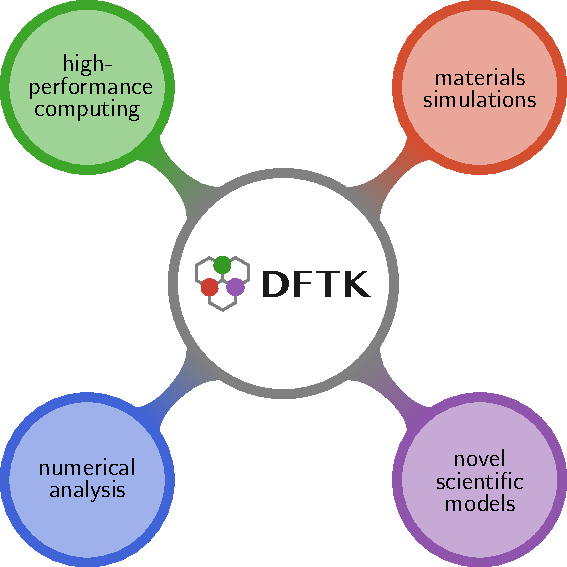
\includegraphics[width=4.6cm]{dftk.pdf}}
    \caption{The multidisciplinary
        directions of research in density-functional theory
        for which DFTK provides a joint software platform.}
    \label{fig:logodftk}
\end{figure}

\section{Acknowledgements} This project has received funding from the Institute of
Computing and Data Sciences (ISCD, Sorbonne Université), École des Ponts
ParisTech, Inria Research Centre Paris and from the European Research Council
(ERC) under the European Union's Horizon 2020 research and innovation program
(grant agreement No 810367).

\bibliographystyle{juliacon}
\bibliography{ref}

% \vadjust{\vfill\pagebreak}
\end{document}
